% Options for packages loaded elsewhere
\PassOptionsToPackage{unicode}{hyperref}
\PassOptionsToPackage{hyphens}{url}
\PassOptionsToPackage{dvipsnames,svgnames,x11names}{xcolor}
%
\documentclass[
  11pt,
]{article}

\usepackage{amsmath,amssymb}
\usepackage[]{libertine}
\usepackage{setspace}
\usepackage{iftex}
\ifPDFTeX
  \usepackage[T1]{fontenc}
  \usepackage[utf8]{inputenc}
  \usepackage{textcomp} % provide euro and other symbols
\else % if luatex or xetex
  \usepackage{unicode-math}
  \defaultfontfeatures{Scale=MatchLowercase}
  \defaultfontfeatures[\rmfamily]{Ligatures=TeX,Scale=1}
  \setmonofont[]{inconsolata}
\fi
% Use upquote if available, for straight quotes in verbatim environments
\IfFileExists{upquote.sty}{\usepackage{upquote}}{}
\IfFileExists{microtype.sty}{% use microtype if available
  \usepackage[]{microtype}
  \UseMicrotypeSet[protrusion]{basicmath} % disable protrusion for tt fonts
}{}
\usepackage{xcolor}
\usepackage[margin = 1in]{geometry}
\setlength{\emergencystretch}{3em} % prevent overfull lines
\setcounter{secnumdepth}{5}
% Make \paragraph and \subparagraph free-standing
\ifx\paragraph\undefined\else
  \let\oldparagraph\paragraph
  \renewcommand{\paragraph}[1]{\oldparagraph{#1}\mbox{}}
\fi
\ifx\subparagraph\undefined\else
  \let\oldsubparagraph\subparagraph
  \renewcommand{\subparagraph}[1]{\oldsubparagraph{#1}\mbox{}}
\fi


\providecommand{\tightlist}{%
  \setlength{\itemsep}{0pt}\setlength{\parskip}{0pt}}\usepackage{longtable,booktabs,array}
\usepackage{calc} % for calculating minipage widths
% Correct order of tables after \paragraph or \subparagraph
\usepackage{etoolbox}
\makeatletter
\patchcmd\longtable{\par}{\if@noskipsec\mbox{}\fi\par}{}{}
\makeatother
% Allow footnotes in longtable head/foot
\IfFileExists{footnotehyper.sty}{\usepackage{footnotehyper}}{\usepackage{footnote}}
\makesavenoteenv{longtable}
\usepackage{graphicx}
\makeatletter
\def\maxwidth{\ifdim\Gin@nat@width>\linewidth\linewidth\else\Gin@nat@width\fi}
\def\maxheight{\ifdim\Gin@nat@height>\textheight\textheight\else\Gin@nat@height\fi}
\makeatother
% Scale images if necessary, so that they will not overflow the page
% margins by default, and it is still possible to overwrite the defaults
% using explicit options in \includegraphics[width, height, ...]{}
\setkeys{Gin}{width=\maxwidth,height=\maxheight,keepaspectratio}
% Set default figure placement to htbp
\makeatletter
\def\fps@figure{htbp}
\makeatother

\usepackage{booktabs}
\usepackage{longtable}
\usepackage{array}
\usepackage{multirow}
\usepackage{wrapfig}
\usepackage{float}
\usepackage{colortbl}
\usepackage{pdflscape}
\usepackage{tabu}
\usepackage{threeparttable}
\usepackage{threeparttablex}
\usepackage[normalem]{ulem}
\usepackage{makecell}
\usepackage{xcolor}
\onehalfspacing
\makeatletter
\makeatother
\makeatletter
\makeatother
\makeatletter
\@ifpackageloaded{caption}{}{\usepackage{caption}}
\AtBeginDocument{%
\ifdefined\contentsname
  \renewcommand*\contentsname{Table of contents}
\else
  \newcommand\contentsname{Table of contents}
\fi
\ifdefined\listfigurename
  \renewcommand*\listfigurename{List of Figures}
\else
  \newcommand\listfigurename{List of Figures}
\fi
\ifdefined\listtablename
  \renewcommand*\listtablename{List of Tables}
\else
  \newcommand\listtablename{List of Tables}
\fi
\ifdefined\figurename
  \renewcommand*\figurename{Figure}
\else
  \newcommand\figurename{Figure}
\fi
\ifdefined\tablename
  \renewcommand*\tablename{Table}
\else
  \newcommand\tablename{Table}
\fi
}
\@ifpackageloaded{float}{}{\usepackage{float}}
\floatstyle{ruled}
\@ifundefined{c@chapter}{\newfloat{codelisting}{h}{lop}}{\newfloat{codelisting}{h}{lop}[chapter]}
\floatname{codelisting}{Listing}
\newcommand*\listoflistings{\listof{codelisting}{List of Listings}}
\makeatother
\makeatletter
\@ifpackageloaded{caption}{}{\usepackage{caption}}
\@ifpackageloaded{subcaption}{}{\usepackage{subcaption}}
\makeatother
\makeatletter
\@ifpackageloaded{tcolorbox}{}{\usepackage[many]{tcolorbox}}
\makeatother
\makeatletter
\@ifundefined{shadecolor}{\definecolor{shadecolor}{rgb}{.97, .97, .97}}
\makeatother
\makeatletter
\makeatother
\ifLuaTeX
  \usepackage{selnolig}  % disable illegal ligatures
\fi
\usepackage[style = windycity,reflist,autocite = inline,backend =
biber,url = false,doi = false,isbn = false]{biblatex}
\addbibresource{references.bib}
\IfFileExists{bookmark.sty}{\usepackage{bookmark}}{\usepackage{hyperref}}
\IfFileExists{xurl.sty}{\usepackage{xurl}}{} % add URL line breaks if available
\urlstyle{same} % disable monospaced font for URLs
\hypersetup{
  pdftitle={Blues in Colors: Police Violence, Racial Representation, and White Attitude Change},
  pdfauthor={Chaoyue Wang},
  colorlinks=true,
  linkcolor={DeepSkyBlue4},
  filecolor={Maroon},
  citecolor={DodgerBlue4},
  urlcolor={SpringGreen4},
  pdfcreator={LaTeX via pandoc}}

\title{\textbf{Blues in Colors: Police Violence, Racial Representation,
and White Attitude Change}}
\author{Chaoyue Wang}
\date{October 3, 2022}

\begin{document}
\maketitle
\begin{abstract}
Political behavior has been structured along group identities, and a
racial division emerges regarding attitudes toward law enforcement and
actions on police brutality. Compared to people of color, white
Americans are more supportive of police agencies and more hesitant about
reforming policing behavior even in the wake of multiple recent
unjustified police-involved homicides. While existing studies attribute
such difference to white's unique experiences with law enforcement,
excessive white representation in police workforces has received little
attention. Linking a nationally representative sample to their local
context of racialized police and police violence, this study finds that
more representation of black and Hispanic officers greatly enhances the
process where white residents reacts to police violence by holding more
critical view toward law enforcement. Interestingly, white
representation in police has only weak effect of such. Findings here
highlights group thinking as a contributing factor to today's racial
divide on policing, and implicates how promoting racial diversity in
police workforce can facilitate the outset of meaningful conversations
on police violence.
\end{abstract}
\captionsetup{labelfont = {bf,},font = small}

\ifdefined\Shaded\renewenvironment{Shaded}{\begin{tcolorbox}[boxrule=0pt, borderline west={3pt}{0pt}{shadecolor}, frame hidden, breakable, enhanced, interior hidden, sharp corners]}{\end{tcolorbox}}\fi

\setstretch{1.5}
\hypertarget{empirical-strategy}{%
\section{Empirical Strategy}\label{empirical-strategy}}

The challenging nature of political behavior writing lies upon not the
quantity and complexity demanded for organizing a richly textured yet
rigorously ordered narrative, like that in the discipline of historical
and cultural analysis, but the rarity, even among the most polished
writings in this profession, of a masterful balance of empirical
indications and theoretical interpretations where raw, lukewarm data and
their statistical derivatives are smoothly situated within a context of
vivid, vibrant ideas \autocite{egan2020,mason2018,abrajano2015}.

Political behavior has been structured along group identities, and a
racial division emerges regarding attitudes toward law enforcement and
actions on police brutality. Compared to people of color, white
Americans are more supportive of police agencies and more hesitant about
reforming policing behavior even in the wake of multiple recent
unjustified police-involved homicides. While existing studies attribute
such difference to white's unique experiences with law enforcement,
excessive white representation in police workforce has received little
attention. Linking a nationally representative sample to their local
context of racialized police and police violence, this study finds that
more representation of black and Hispanic officers greatly enhances the
process where white residents reacts to police violence by holding more
critical view toward law enforcement. Interestingly, white
representation in police has only weak effect of such. Findings here
highlights group thinking as a contributing factor to today's racial
divide on policing, and implicates how promoting racial diversity in
police workforce can facilitate the outset of meaningful conversations
on police violence.

\begin{figure}[t]

{\centering 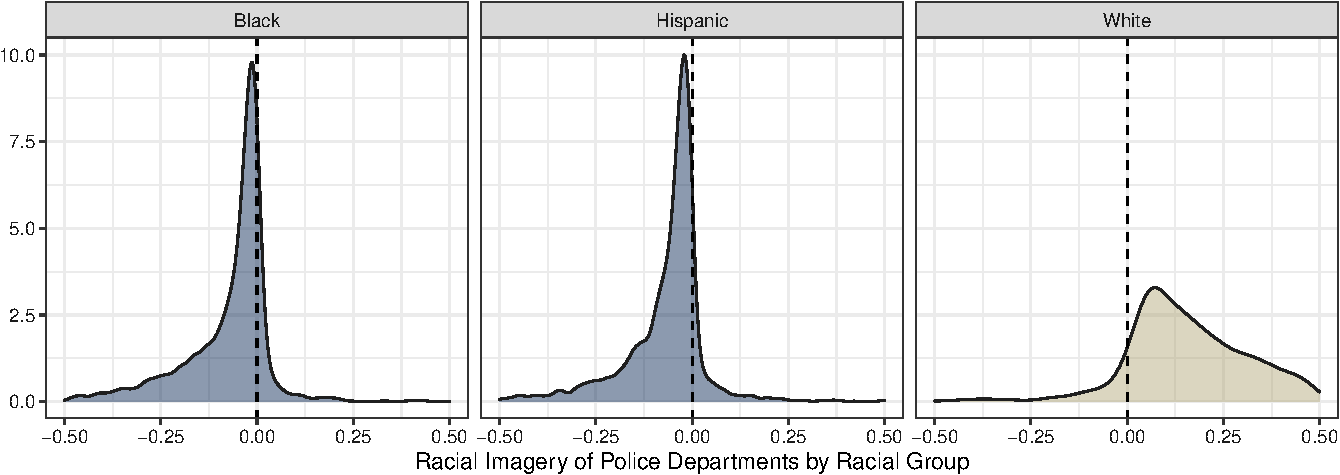
\includegraphics{paper_files/figure-pdf/fig-lemas-density-1.pdf}

}

\caption{\label{fig-lemas-density}\textbf{Distribution of Racial
Presence among Police Departments Surveyed in LEMAS 2016.} On the
horizontal axis, a positive value indicates that the corresponding
racial group is excessively represented in local police departments, and
a negative value the otherwise.}

\end{figure}

\begin{figure}[t]

{\centering 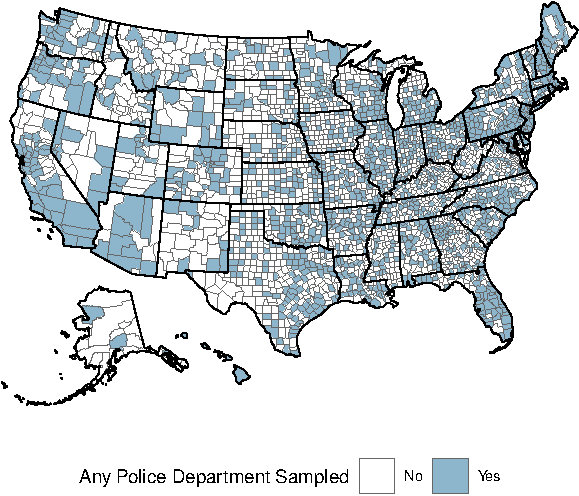
\includegraphics{paper_files/figure-pdf/fig-lemas-cover-1.pdf}

}

\caption{\label{fig-lemas-cover}\textbf{Geographic Coverage of LEMAS
2016 at the County Level.} Counties are colored blue where at least one
police department within its jurisdiction is surveyed in LEMAS 2016.}

\end{figure}

\begin{figure}[t]

{\centering 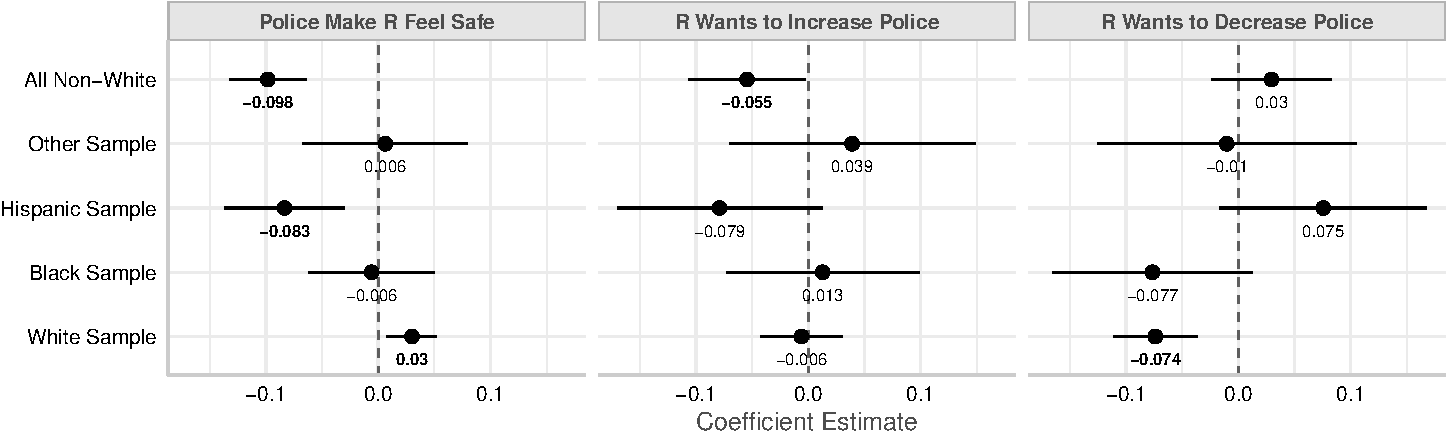
\includegraphics{paper_files/figure-pdf/fig-baseline-1.pdf}

}

\caption{\label{fig-baseline}\textbf{the Estiamted Relationship between
Racial Imagery of Local Police and White Attitudes on Policing.} Linear
predicted values of outcome attitudes are based upon the previous
interactional OLS model.}

\end{figure}

\hypertarget{tbl-divides}{}
\begin{table}
\caption{\label{tbl-divides}Racial Imagery of Local Police Moderates Racial Divides on Police
Violence. }\tabularnewline

\centering
\begin{tabular}[t]{lccc}
\toprule
  & Police Felt as Safe & Increase Police & Decrease Police\\
\midrule
\cellcolor{gray!6}{Racial Divide} & \cellcolor{gray!6}{0.221***} & \cellcolor{gray!6}{0.048**} & \cellcolor{gray!6}{-0.072***}\\
 & (0.016) & (0.016) & (0.016)\\
\cellcolor{gray!6}{White Imagery of Police} & \cellcolor{gray!6}{-0.168***} & \cellcolor{gray!6}{0.003} & \cellcolor{gray!6}{0.018}\\
 & (0.049) & (0.048) & (0.048)\\
\cellcolor{gray!6}{Racial Divide × White Imagery} & \cellcolor{gray!6}{0.182**} & \cellcolor{gray!6}{0.019} & \cellcolor{gray!6}{-0.039}\\
 & (0.055) & (0.057) & (0.055)\\
\midrule
\cellcolor{gray!6}{Num.Obs.} & \cellcolor{gray!6}{39551} & \cellcolor{gray!6}{39597} & \cellcolor{gray!6}{39589}\\
R2 & 0.076 & 0.002 & 0.007\\
\bottomrule
\multicolumn{4}{l}{\rule{0pt}{1em}This is the note of your regression table.}\\
\multicolumn{4}{l}{\rule{0pt}{1em}+ p $<$ 0.1, * p $<$ 0.05, ** p $<$ 0.01, *** p $<$ 0.001}\\
\end{tabular}
\end{table}

\begin{figure}[t]

{\centering 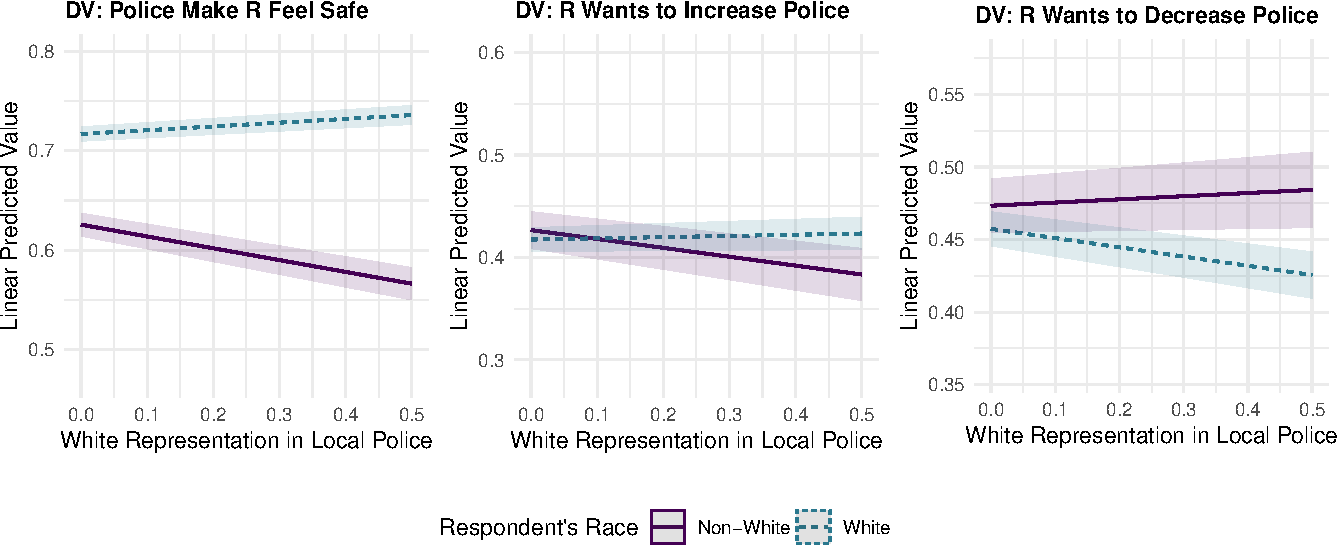
\includegraphics{paper_files/figure-pdf/fig-divides-1.pdf}

}

\caption{\label{fig-divides}\textbf{Racial Imagery of Local Police
Moderates Whites' Attitudinal Response to Police Violence.} Linear
predicted values of outcome attitudes are based upon the previous
interactional OLS model.}

\end{figure}

\hypertarget{tbl-reaction}{}
\begin{table}
\caption{\label{tbl-reaction}Racial Imagery of Local Police Moderates Racial Reaction to Police
Violence. }\tabularnewline

\centering
\begin{tabular}[t]{lccc}
\toprule
  & Police Felt as Safe & Increase Police & Decrease Police\\
\midrule
\cellcolor{gray!6}{White Imagery of Police} & \cellcolor{gray!6}{0.009} & \cellcolor{gray!6}{-0.009} & \cellcolor{gray!6}{-0.014}\\
 & (0.027) & (0.029) & (0.029)\\
\cellcolor{gray!6}{Any Police Violence in 2020} & \cellcolor{gray!6}{-0.070***} & \cellcolor{gray!6}{-0.057***} & \cellcolor{gray!6}{0.074***}\\
 & (0.012) & (0.013) & (0.013)\\
\cellcolor{gray!6}{Police Violence × White Imagery} & \cellcolor{gray!6}{0.130**} & \cellcolor{gray!6}{0.078+} & \cellcolor{gray!6}{-0.142**}\\
 & (0.041) & (0.045) & (0.045)\\
\midrule
\cellcolor{gray!6}{Num.Obs.} & \cellcolor{gray!6}{26016} & \cellcolor{gray!6}{26039} & \cellcolor{gray!6}{26036}\\
R2 & 0.004 & 0.002 & 0.003\\
\bottomrule
\multicolumn{4}{l}{\rule{0pt}{1em}This is the note of your regression table.}\\
\multicolumn{4}{l}{\rule{0pt}{1em}+ p $<$ 0.1, * p $<$ 0.05, ** p $<$ 0.01, *** p $<$ 0.001}\\
\end{tabular}
\end{table}

\begin{figure}[t]

{\centering 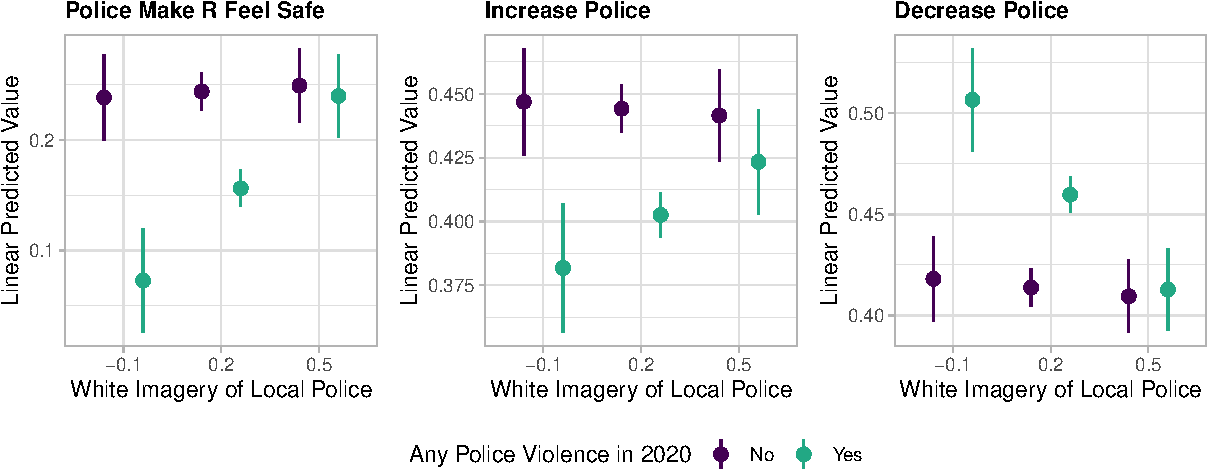
\includegraphics{paper_files/figure-pdf/fig-reaction-mod-1.pdf}

}

\caption{\label{fig-reaction-mod}\textbf{Racial Imagery of Local Police
Moderates Whites' Attitudinal Response to Police Violence.} Linear
predicted values of outcome attitudes are based upon the previous
interactional OLS model.}

\end{figure}

\begin{figure}[t]

{\centering 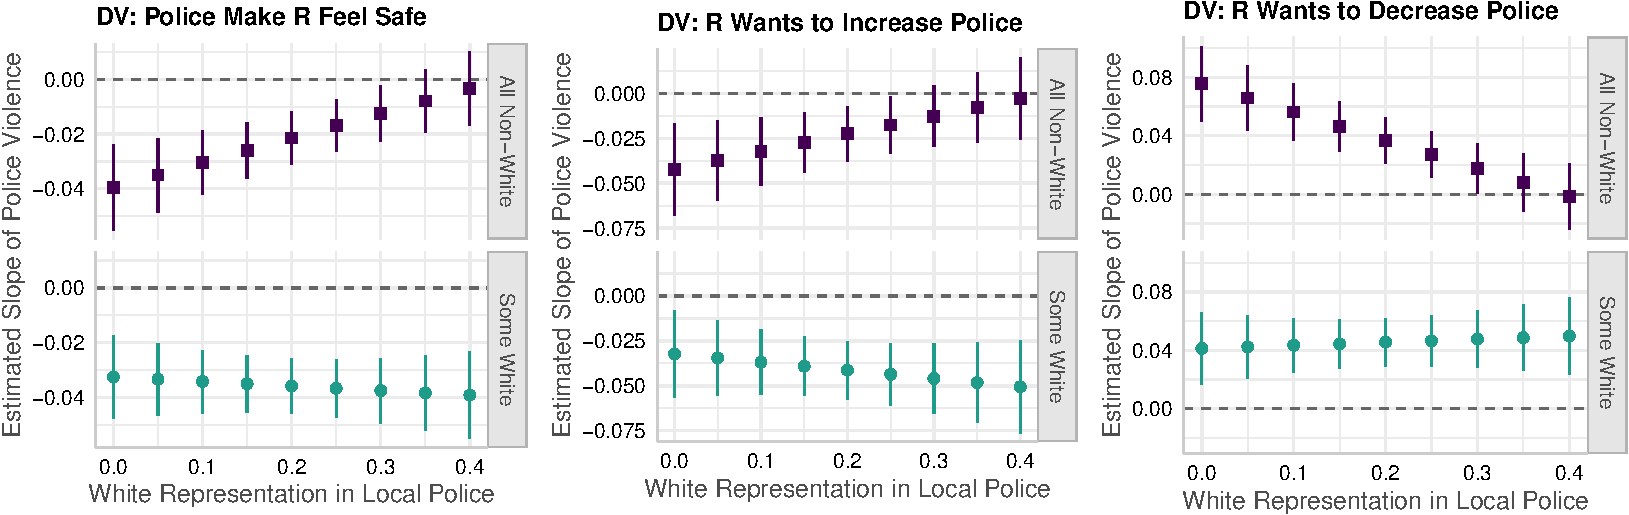
\includegraphics{paper_files/figure-pdf/fig-racial-component-1.pdf}

}

\caption{\label{fig-racial-component}\textbf{Racial Imagery of Local
Police Moderates Whites' Attitudinal Response to Police Violence.}
Linear predicted values of outcome attitudes are based upon the previous
interactional OLS model.}

\end{figure}

\hypertarget{tbl-racial.component}{}
\begin{table}
\caption{\label{tbl-racial.component}Racial Imagery of Local Police Moderates Whites' Attitudinal Response to
Police Violence. }\tabularnewline

\centering
\begin{tabular}[t]{lccc}
\toprule
  & Police Felt as Safe & Increase Police & Decrease Police\\
\midrule
\cellcolor{gray!6}{White Imagery of Police} & \cellcolor{gray!6}{0.007} & \cellcolor{gray!6}{-0.013} & \cellcolor{gray!6}{-0.010}\\
 & (0.027) & (0.029) & (0.029)\\
\cellcolor{gray!6}{PV Whites} & \cellcolor{gray!6}{-0.065***} & \cellcolor{gray!6}{-0.039*} & \cellcolor{gray!6}{0.056***}\\
 & (0.015) & (0.016) & \vphantom{1} (0.016)\\
\cellcolor{gray!6}{PV POC} & \cellcolor{gray!6}{-0.076***} & \cellcolor{gray!6}{-0.077***} & \cellcolor{gray!6}{0.093***}\\
 & (0.015) & (0.016) & (0.016)\\
\cellcolor{gray!6}{White Imagery × PV Whites} & \cellcolor{gray!6}{0.098+} & \cellcolor{gray!6}{-0.003} & \cellcolor{gray!6}{-0.075}\\
 & (0.053) & (0.057) & (0.057)\\
\cellcolor{gray!6}{White Imagery × PV POC} & \cellcolor{gray!6}{0.164**} & \cellcolor{gray!6}{0.162**} & \cellcolor{gray!6}{-0.210***}\\
 & (0.053) & (0.058) & (0.058)\\
\midrule
\cellcolor{gray!6}{Num.Obs.} & \cellcolor{gray!6}{26016} & \cellcolor{gray!6}{26039} & \cellcolor{gray!6}{26036}\\
R2 & 0.004 & 0.002 & 0.003\\
\bottomrule
\multicolumn{4}{l}{\rule{0pt}{1em}This is the note of your regression table.}\\
\multicolumn{4}{l}{\rule{0pt}{1em}+ p $<$ 0.1, * p $<$ 0.05, ** p $<$ 0.01, *** p $<$ 0.001}\\
\end{tabular}
\end{table}


\printbibliography[title=References]


\end{document}
